\documentclass[11pt,a4paper]{article}
\usepackage[margin=22mm]{geometry}
\usepackage[T1]{fontenc}
\usepackage[utf8]{inputenc}
\usepackage{lmodern}
\usepackage{xcolor}
\usepackage{booktabs}
\usepackage{tabularx}
\usepackage{array}
\usepackage{enumitem}
\usepackage{hyperref}
\usepackage{listings}
\usepackage{fancyhdr}
\usepackage{tikz}
\usetikzlibrary{arrows.meta,positioning,shapes.geometric}

\definecolor{Ink}{HTML}{172033}
\definecolor{Blue}{HTML}{3157D5}
\definecolor{Teal}{HTML}{168A83}
\definecolor{Soft}{HTML}{F2F5FA}
\definecolor{Muted}{HTML}{5D6678}
\definecolor{Danger}{HTML}{A43B3B}
\hypersetup{colorlinks=true,linkcolor=Blue,urlcolor=Blue}
\pagestyle{fancy}
\fancyhf{}
\lhead{Task 1 explained}
\rhead{SuperDocs growth machine}
\cfoot{\thepage}
\setlength{\parindent}{0pt}
\setlength{\parskip}{6pt}
\setlist[itemize]{leftmargin=18pt,itemsep=3pt,topsep=3pt}
\setlist[enumerate]{leftmargin=20pt,itemsep=3pt,topsep=3pt}
\lstset{basicstyle=\ttfamily\small,backgroundcolor=\color{Soft},frame=single,rulecolor=\color{Soft},breaklines=true,columns=fullflexible}
\newcommand{\pathcode}[1]{\texttt{#1}}
\newcommand{\keypoint}[1]{\textcolor{Blue}{\textbf{#1}}}

\title{\vspace{-18mm}\textbf{Task 1: Founder Doc Signal Machine}\\[4pt]\large What it is, how it works, what the evidence means, and how n8n fits}
\author{Repository walkthrough}
\date{10 August 2026}

\begin{document}
\maketitle
\thispagestyle{empty}

\begin{center}
\colorbox{Soft}{\parbox{0.91\textwidth}{
\textbf{One-sentence explanation.} Task 1 is an offline, draft-only growth system that turns a human-researched CSV of small B2B founder prospects into claim-checked, personalized Markdown outreach drafts and a reproducible evidence bundle. It intentionally never sends anything.
}}
\end{center}

\vfill
\textbf{The most important distinction}

This is not an autonomous lead scraper and it is not an email campaign. Humans find and research candidate companies. Automation begins only after a structured CSV has been prepared. The machine validates that input, maps each prospect's document pain to a relevant SuperDocs angle, generates a draft, checks product claims, and records evidence.

\textbf{Included addition}

An importable n8n workflow has been added under \pathcode{n8n/}. It acts as a visual control plane around the existing Python implementation. It does not rewrite or replace the original machine.

\newpage
\tableofcontents
\newpage

\section{Why Task 1 exists}

The assignment requires a growth machine with four parts: a defensible audience, a runnable system executed twice, an audience-facing piece, and honest measurement. The repository meets that shape as follows:

\begin{tabularx}{\textwidth}{>{\bfseries}p{0.24\textwidth} X}
\toprule
Requirement & Where it appears \\
\midrule
Audience & \pathcode{AUDIENCE.md} defines one narrow behavioral group and a method for finding initial companies. \\
Runnable system & \pathcode{machine/} contains the Python pipeline; \pathcode{data/} contains two input batches. \\
Two executions & \pathcode{runs/run-1/}, \pathcode{runs/run-2/}, and corresponding \pathcode{outbox/} folders preserve evidence. \\
Audience-facing piece & \pathcode{piece/index.html} is a focused landing page for the selected audience. \\
Measurement & \pathcode{MEASUREMENT.md} explains what was measured, what changed, and what cannot honestly be claimed. \\
\bottomrule
\end{tabularx}

The selected audience is not ``all SaaS companies.'' It is seed-stage technical founders and founding engineers at roughly 2--25 person B2B product companies who already use coding agents but still personally finish proposals, updates, questionnaires, policy packs, or one-pagers by hand.

The core insight is: \keypoint{chat may solve the words, while the document handoff remains manual}. SuperDocs is positioned as closing that last mile by editing the actual document with review, history, and style-preserving export.

\section{The complete flow}

\begin{center}
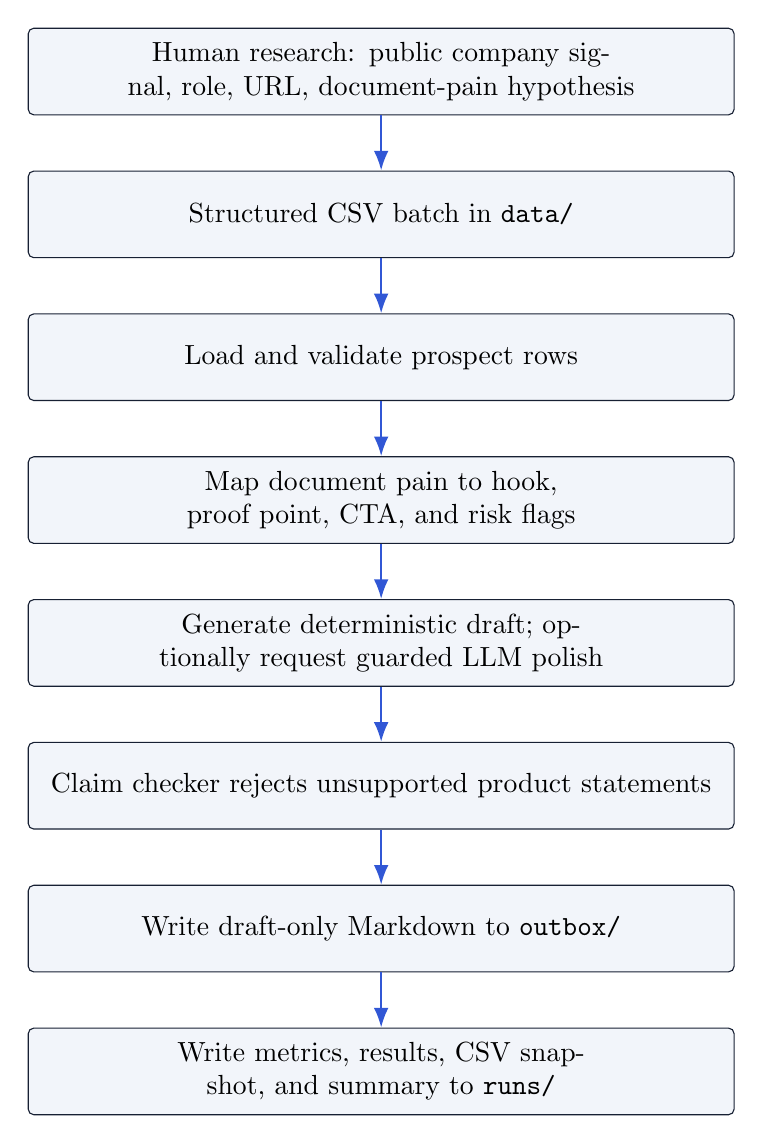
\begin{tikzpicture}[
  node distance=7mm,
  box/.style={draw=Ink, rounded corners=2pt, fill=Soft, text width=0.72\textwidth, minimum height=11mm, align=center},
  arrow/.style={-{Latex[length=2.5mm]}, thick, draw=Blue}
]
\node[box] (research) {Human research: public company signal, role, URL, document-pain hypothesis};
\node[box, below=of research] (csv) {Structured CSV batch in \texttt{data/}};
\node[box, below=of csv] (load) {Load and validate prospect rows};
\node[box, below=of load] (enrich) {Map document pain to hook, proof point, CTA, and risk flags};
\node[box, below=of enrich] (draft) {Generate deterministic draft; optionally request guarded LLM polish};
\node[box, below=of draft] (claims) {Claim checker rejects unsupported product statements};
\node[box, below=of claims] (write) {Write draft-only Markdown to \texttt{outbox/}};
\node[box, below=of write] (evidence) {Write metrics, results, CSV snapshot, and summary to \texttt{runs/}};
\draw[arrow] (research)--(csv);
\draw[arrow] (csv)--(load);
\draw[arrow] (load)--(enrich);
\draw[arrow] (enrich)--(draft);
\draw[arrow] (draft)--(claims);
\draw[arrow] (claims)--(write);
\draw[arrow] (write)--(evidence);
\end{tikzpicture}
\end{center}

The boundary before the CSV matters. The system does not browse the web and does not discover private contact data. A person must inspect public material and formulate the research fields first.

\section{Folder-by-folder explanation}

\subsection{The strategy documents}

\textbf{\pathcode{AUDIENCE.md}} answers who the machine is for, why that audience is plausible, what their current workflow looks like, and how the first companies would be found. It also lists explicit cuts, such as broad SMB targeting, enterprise IT, generic creators, and real outreach during this task.

\textbf{\pathcode{MEASUREMENT.md}} prevents the machine from pretending that drafts are campaign results. Because sending is prohibited, the valid measures are production measures: valid rows, completed drafts, claim safety, research risk flags, reproducibility, and batch overlap.

\textbf{\pathcode{README.md}} is the concise operating entry point. It gives the reproducible commands and points to the evidence.

\subsection{The inputs: \pathcode{data/}}

There are two CSV batches with eight synthetic companies each. Every row represents a company-role pair, not a named private person. Important fields include:

\begin{tabularx}{\textwidth}{>{\ttfamily}p{0.28\textwidth} X}
\toprule
\normalfont\textbf{Field} & \textbf{Purpose} \\
\midrule
prospect\_id & Stable safe identifier used in output file names. \\
company, role & Company and role-level targeting without storing a personal name. \\
public\_signal, public\_url & Where the research hypothesis came from. \\
product\_one\_liner & Short description of the prospect's product. \\
doc\_pain & Category such as proposal, investor update, policy pack, or questionnaire. \\
recent\_public\_detail & Specific context used to avoid a generic opening. \\
hypothesis & The document-workflow pain being tested. \\
is\_synthetic & Distinguishes synthetic rows and supports risk flagging. \\
\bottomrule
\end{tabularx}

\subsection{The code: \pathcode{machine/}}

\textbf{\pathcode{config.py}} defines paths, the product description, allowed capability claims, forbidden claim fragments, optional OpenAI configuration, and the hard safety switch \pathcode{SEND\_MODE = False}.

\textbf{\pathcode{prospects.py}} parses CSV files into typed prospect objects. It requires the expected columns, rejects duplicate IDs, rejects unsafe IDs, ignores blank rows, and preserves additional CSV fields.

\textbf{\pathcode{enrich.py}} performs deterministic enrichment. A playbook maps document pain to four pieces: a pain label, hook angle, proof point, and restrained CTA. It also adds flags for thin research, missing URLs, non-synthetic rows, or a weak product description.

\textbf{\pathcode{personalize.py}} creates a deterministic draft first. If LLM use is enabled and an API key exists, it asks OpenAI for a shorter polish under strict rules. Any API error, malformed response, excessive length, or failed claim check causes a fallback to the deterministic draft.

\textbf{\pathcode{run.py}} orchestrates the batch. It creates output directories, clears old files for the selected run ID, processes each prospect, writes Markdown drafts, creates metrics and detailed result JSON, snapshots the input CSV, and writes a readable run summary.

\subsection{The outputs: \pathcode{outbox/} and \pathcode{runs/}}

Each file in \pathcode{outbox/<run-id>/} is Markdown with front matter that explicitly records \pathcode{send\_mode: false} and \pathcode{status: DRAFT\_ONLY\_NOT\_SENT}. The message addresses a role at a company rather than inventing a person's name.

Each \pathcode{runs/<run-id>/} folder contains:

\begin{itemize}
  \item \pathcode{metrics.json}: aggregate operational measures;
  \item \pathcode{results.json}: one record per prospect, including claim-check and risk details;
  \item \pathcode{batch.snapshot.csv}: the exact batch used for reproducibility;
  \item \pathcode{SUMMARY.md}: a readable index of the generated drafts.
\end{itemize}

\subsection{The public piece: \pathcode{piece/index.html}}

The landing page translates the audience hypothesis into audience-facing language. Its message is that the coding agent created a draft, but the founder still has to transfer it into a reviewed, styled customer document. The page contrasts the current paste-and-repair loop with a direct document-editing loop and highlights proposals, investor updates, and related workflows.

\section{Safety and quality controls}

\begin{tabularx}{\textwidth}{>{\bfseries}p{0.31\textwidth} X}
\toprule
Control & What it prevents \\
\midrule
Hard-coded no-send mode & The machine refuses to run if \pathcode{SEND\_MODE} becomes true. No sending integration exists. \\
Safe run and prospect IDs & Blocks path traversal through identifiers used in file paths. \\
Company + role targeting & Avoids storing or fabricating private personal names. \\
Allowed/forbidden claims & Keeps SuperDocs statements within documented present capabilities. \\
Product-scoped claim check & Prospect context such as a public SOC2 journey is not falsely treated as a SuperDocs compliance claim. \\
Deterministic fallback & Makes production reproducible and protects against model or network failure. \\
Input snapshot & Makes each run auditable against its exact source rows. \\
Regression tests & Preserve fixes for claim scope and path-safety behavior. \\
\bottomrule
\end{tabularx}

One subtle correction is documented in \pathcode{MEASUREMENT.md}: an early claim checker treated a prospect's SOC2 context as though it were a SuperDocs claim. The checker was narrowed to the subject and product-related part of the message, then regression tests were added. This is useful evidence of iteration because the failure was found, understood, fixed, and preserved in tests.

\section{What the two recorded runs mean}

\begin{tabular}{lrrr}
\toprule
Metric & Run 1 & Run 2 & Combined \\
\midrule
Fresh prospects & 8 & 8 & 16 \\
Drafts written & 8 & 8 & 16 \\
Completion rate & 100\% & 100\% & 100\% \\
Claim-check failures & 0 & 0 & 0 \\
Rows with risk flags & 0 & 0 & 0 \\
Emails sent & 0 & 0 & 0 \\
Batch overlap & -- & 0 & 0 \\
\bottomrule
\end{tabular}

These numbers establish that the offline system processed two fresh batches completely and reproducibly under its current checks. They do \textbf{not} establish message-market fit, reply rate, meeting rate, or revenue impact. Those outcomes cannot exist without permitted, human-reviewed outreach.

A future experiment is already scoped responsibly: manually review five drafts and compare one framing variable, while guarding claim accuracy and negative-response risk. That is a next step, not a result claimed by this submission.

\section{How the n8n workflow fits}

The added file \pathcode{n8n/task-1-growth-machine.workflow.json} provides a visual orchestration layer:

\begin{enumerate}
  \item \textbf{Manual Trigger} ensures a person deliberately starts the run.
  \item \textbf{Workflow Configuration} sets the mounted project path, CSV batch, safe run ID, and LLM choice.
  \item \textbf{Validate and Build Command} rejects traversal and unsafe identifiers, then constructs the command.
  \item \textbf{Run Existing Python Machine} executes the original implementation through n8n's Execute Command node.
  \item \textbf{Safety Gate and Run Summary} parses metrics and fails unless sending stayed off, emails sent stayed at zero, all accepted rows produced drafts, and claim-check failures stayed at zero.
\end{enumerate}

\begin{center}
\colorbox{Soft}{\parbox{0.91\textwidth}{
\textbf{Why wrap instead of rewrite?} Reimplementing the logic in JavaScript nodes would create two sources of truth that could drift. The wrapper preserves the tested Python behavior while giving an n8n-oriented operator a visual trigger, configuration surface, execution history, and explicit final gate.
}}
\end{center}

The workflow requires self-hosted n8n because Execute Command is not available in n8n Cloud. The Task 1 directory must be mounted read-write into the n8n runtime because a run creates drafts and evidence. Detailed import and Docker instructions are in \pathcode{n8n/README.md}.

\section{How to run the original machine}

From \pathcode{task-1-growth-machine/}:

\begin{lstlisting}
python3 -m machine.run --batch data/batch-1.csv --run-id run-1 --no-llm
python3 -m machine.run --batch data/batch-2.csv --run-id run-2 --no-llm
python3 -m unittest discover -s tests -v
\end{lstlisting}

For a new non-destructive review run, use a fresh ID rather than \pathcode{run-1} or \pathcode{run-2}, because the machine intentionally clears existing draft files inside the selected outbox run directory before regenerating them.

Example:

\begin{lstlisting}
python3 -m machine.run \
  --batch data/batch-1.csv \
  --run-id review-run \
  --no-llm
\end{lstlisting}

\section{Strengths, limits, and practical interpretation}

\textbf{Strengths}
\begin{itemize}
  \item The audience is behaviorally specific and tied to the product's real wedge.
  \item The system is small, runnable, reproducible, and evidenced twice.
  \item Safety constraints are implemented in code rather than left as prose.
  \item Deterministic generation makes review and debugging straightforward.
  \item The measurement document distinguishes operational success from market success.
\end{itemize}

\textbf{Current limits}
\begin{itemize}
  \item Research collection is manual and the supplied companies are synthetic.
  \item The claim checker is rule-based, so it can miss unsupported wording that does not match its fragments or markers.
  \item A completed draft is not proof that a human would find the message relevant or well written.
  \item Risk flags are soft signals; they do not replace human review of non-synthetic research.
  \item The n8n wrapper depends on self-hosting and access to the local Python project.
\end{itemize}

\textbf{Bottom line}

Task 1 is best understood as a carefully bounded production prototype: research enters as structured data, deterministic automation produces safe draft artifacts, and every run leaves an audit trail. It demonstrates that the process can operate reliably. It intentionally stops before the ethically and procedurally prohibited step of contacting anyone.

\section*{Quick reference}

\begin{tabularx}{\textwidth}{>{\bfseries}p{0.30\textwidth} X}
\toprule
Question & Answer \\
\midrule
Does it scrape leads? & No. Human research is completed before the CSV stage. \\
Does it send email? & No. Sending is hard-disabled and absent from both Python and n8n. \\
Does it require an LLM? & No. The recorded runs are deterministic. \\
What does it create? & Markdown drafts plus metrics, results, an input snapshot, and a summary. \\
What proves it ran? & The two \pathcode{runs/} evidence folders and matching \pathcode{outbox/} drafts. \\
What is n8n doing? & Visually configuring, running, and gating the existing Python machine. \\
What remains unproven? & Real-world response, conversion, and market impact. \\
\bottomrule
\end{tabularx}

\end{document}
